% !TEX program = xelatex
% IA712 - Project B: Autonomous Search and Rescue - 10-minute presentation (EN)
\documentclass[aspectratio=169,11pt]{beamer}
\usepackage{amsmath}
\usepackage{fontspec}
\usepackage{graphicx}
\graphicspath{{img/}}
\usepackage{tikz}
\usetikzlibrary{arrows.meta,positioning,shapes.geometric,fit,calc}
\usepackage{booktabs}

\definecolor{nccblue}{HTML}{1F4E79}
\definecolor{nccsky}{HTML}{1F6FEB}
\definecolor{nccorange}{HTML}{FB8500}
\definecolor{nccgreen}{HTML}{2DA44E}
\definecolor{nccred}{HTML}{D1242F}
\definecolor{nccdark}{HTML}{222831}

\usetheme{default}
\usecolortheme{default}
\setbeamercolor{structure}{fg=nccblue}
\setbeamercolor{frametitle}{fg=nccblue}
\setbeamertemplate{frametitle}{\vspace{0.6mm}{\color{nccblue}\large\bfseries\insertframetitle}\par\vspace{0.3mm}}
\setbeamertemplate{navigation symbols}{}
\setbeamertemplate{footline}[frame number]
\setbeamerfont{frametitle}{series=\bfseries}
\setbeamertemplate{itemize items}[circle]
\setbeamercolor{itemize item}{fg=nccorange}
\setbeamercolor{itemize subitem}{fg=nccsky}

\tikzset{
  box/.style={rounded corners=2pt,draw=nccblue,fill=nccblue!6,align=center,inner sep=3pt,font=\scriptsize,minimum height=7mm,text width=20mm},
  phase1/.style={box,fill=nccsky!15,draw=nccsky},
  phase2/.style={box,fill=nccorange!15,draw=nccorange},
  io/.style={box,fill=nccgreen!12,draw=nccgreen},
  proc/.style={box,fill=white},
  btnode/.style={box,fill=nccblue!12,draw=nccblue},
  ar/.style={-{Latex[length=2mm]},draw=nccdark!70,semithick},
  arl/.style={ar,font=\tiny,inner sep=1pt},
}

\title{\textbf{Autonomous Search and Rescue}}
\subtitle{Project~B - IA712 Mobile Robotics, Final Project}
\author{\textbf{Team RobotZ}\\[3pt]{\footnotesize Julien GIMENEZ \quad Hugo FANCHINI \quad Paul CINTRA \quad Yimou ZHANG}}
\institute{\small \texttt{https://github.com/YiZeems/autonomous-search-and-rescue}}
\date{IA712 - Session L18}

\begin{document}

% -- Title --
\begin{frame}[plain]
  \titlepage
  \begin{center}\footnotesize
  ROS\,2 Humble $\cdot$ Ignition Gazebo Fortress $\cdot$ TurtleBot~4 $\cdot$ Nav2 $\cdot$ slam\_toolbox $\cdot$ BehaviorTree.CPP
  \end{center}
\end{frame}

% -- Problem --
\begin{frame}{The mission: autonomous search \& rescue}
  \begin{columns}[T]
  \begin{column}{0.58\linewidth}
  \textbf{Scenario:} a robot explores an unknown disaster zone, finds ``victims'' (AprilTags),
  and reports their global coordinates - \emph{no human input}.
  \smallskip
  \textbf{Requirements we satisfy:}
  {\small\begin{itemize}
    \item Autonomous frontier exploration, map $>90\,\%$
    \item Camera detection to \texttt{map} via \texttt{tf2}
    \item Map quality / loop closure (SLAM)
    \item \textbf{Decision = Behavior Tree, not FSM}
    \item One-click launch
    \item Bonus: greedy vs.\ information-gain
  \end{itemize}}
  \end{column}
  \begin{column}{0.40\linewidth}
  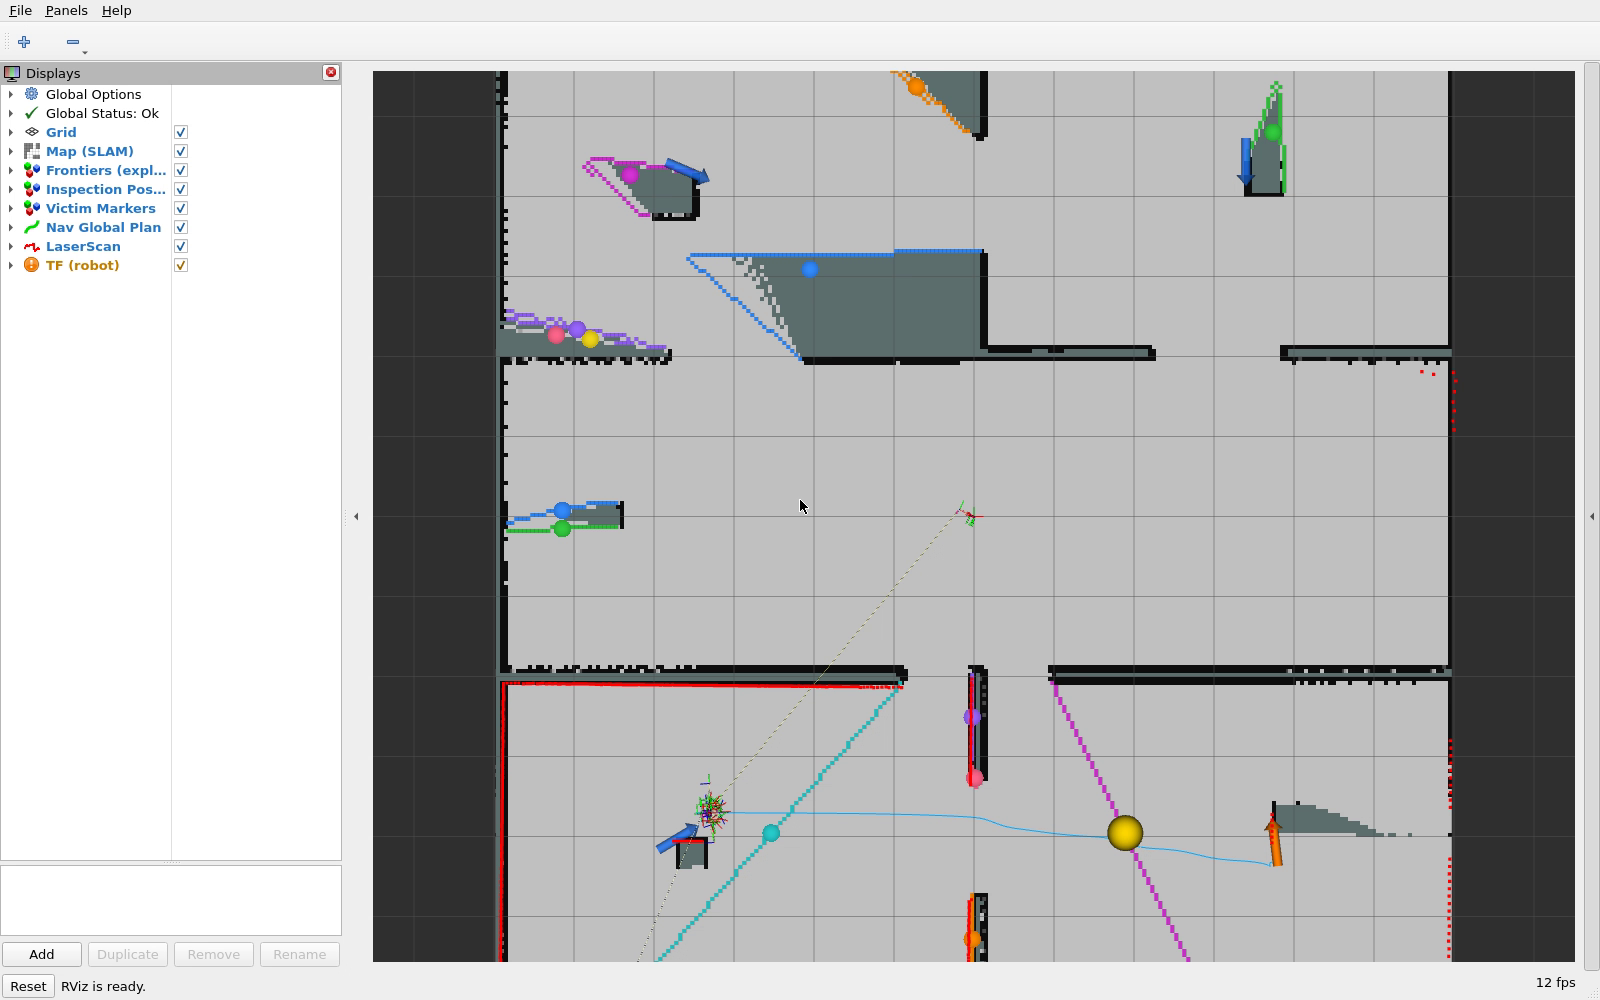
\includegraphics[width=\linewidth]{rviz_live}\\
  {\scriptsize Live RViz: map + 4 victims + algorithms.}
  \end{column}
  \end{columns}
  \vfill
  {\footnotesize\color{nccblue}\textbf{Result:} one continuous autonomous run - \textbf{97.35\,\% coverage, 4/4 victims}.}
\end{frame}

% -- Architecture --
\begin{frame}{System architecture - four ROS\,2 packages}
  \centering
  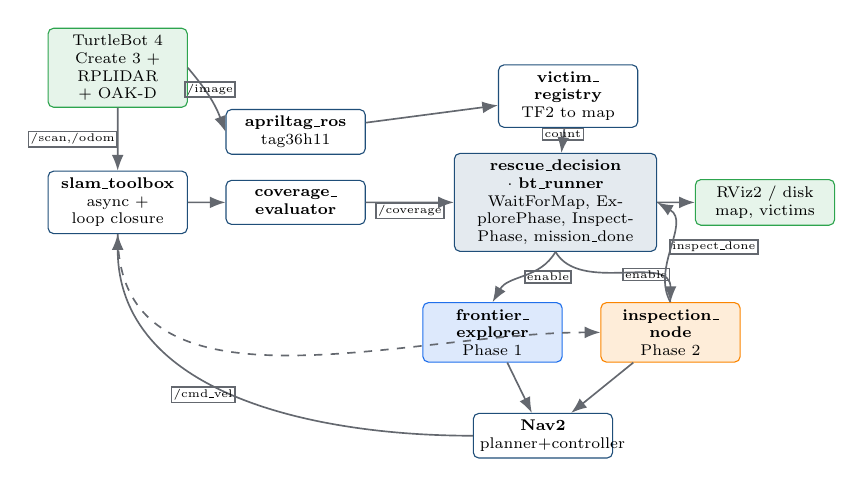
\begin{tikzpicture}[node distance=4mm and 6mm,scale=0.8,transform shape]
    \node[io] (robot) {TurtleBot~4\\\scriptsize Create~3 + RPLIDAR + OAK-D};
    \node[proc,below=10mm of robot] (slam) {\textbf{slam\_toolbox}\\\scriptsize async + loop closure};
    \node[proc,right=of slam] (metric) {\textbf{coverage\_}\\\textbf{evaluator}};
    \node[proc,above=of metric] (april) {\textbf{apriltag\_ros}\\\scriptsize tag36h11};
    \node[btnode,right=14mm of metric,text width=30mm] (bt) {\textbf{rescue\_decision $\cdot$ bt\_runner}\\\scriptsize WaitForMap, ExplorePhase, InspectPhase, mission\_done};
    \node[phase1,below=8mm of bt,xshift=-10mm] (explore) {\textbf{frontier\_}\\\textbf{explorer}\\\scriptsize Phase 1};
    \node[phase2,right=of explore] (inspect) {\textbf{inspection\_}\\\textbf{node}\\\scriptsize Phase 2};
    \node[proc,below=8mm of explore,xshift=8mm] (nav) {\textbf{Nav2}\\\scriptsize planner+controller};
    \node[proc,above=of bt,xshift=2mm] (reg) {\textbf{victim\_}\\\textbf{registry}\\\scriptsize TF2 to map};
    \node[io,right=of bt] (rviz) {RViz2 / disk\\\scriptsize map, victims};
    \draw[ar] (robot) -- node[arl,left]{/scan,/odom} (slam);
    \draw[ar] (robot.east) to[bend left=10] node[arl,above]{/image} (april.west);
    \draw[ar] (slam) -- (metric);
    \draw[ar] (april) -- (reg);
    \draw[ar] (metric) -- node[arl,below]{/coverage} (bt);
    \draw[ar] (bt.south) to[out=-120,in=60] node[arl,right]{enable} (explore.north);
    \draw[ar] (bt.south) to[out=-60,in=90] node[arl,right]{enable} (inspect.north);
    \draw[ar] (inspect.north) to[out=120,in=-30] node[arl,right]{inspect\_done} (bt.east);
    \draw[ar] (explore) -- (nav);
    \draw[ar] (inspect) -- (nav);
    \draw[ar] (nav.west) to[out=180,in=-90] node[arl,left]{/cmd\_vel} (slam.south);
    \draw[ar] (reg) -- node[arl,above]{count} (bt);
    \draw[ar] (bt) -- (rviz);
    \draw[ar,dashed] (slam) to[out=-90,in=180] (inspect.west);
  \end{tikzpicture}
  \par\smallskip
  {\footnotesize The \textbf{Behavior Tree orchestrates}: it gates the Phase~1 explorer and the Phase~2
  inspector via \texttt{/mission/*} topics; the Python nodes do the work. SLAM feeds the map to
  exploration, coverage, Nav2 and inspection.}
\end{frame}

% -- Two-phase BT --
\begin{frame}{Two-phase mission orchestrated by the Behavior Tree}
  \begin{columns}[T]
  \begin{column}{0.36\linewidth}
  \centering
  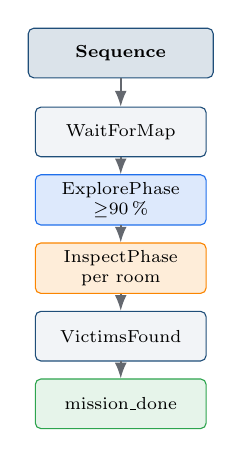
\begin{tikzpicture}[node distance=2.4mm,scale=0.9,transform shape]
    \node[box,fill=nccblue!16,text width=24mm] (root){\textbf{Sequence}};
    \node[box,below=4mm of root,text width=22mm](n1){WaitForMap};
    \node[phase1,below=of n1,text width=22mm](n2){ExplorePhase\\\scriptsize $\geq$90\,\%};
    \node[phase2,below=of n2,text width=22mm](n3){InspectPhase\\\scriptsize per room};
    \node[box,below=of n3,text width=22mm](n4){VictimsFound};
    \node[io,below=of n4,text width=22mm](n5){mission\_done};
    \draw[ar](root)--(n1);\draw[ar](n1)--(n2);\draw[ar](n2)--(n3);\draw[ar](n3)--(n4);\draw[ar](n4)--(n5);
  \end{tikzpicture}
  \end{column}
  \begin{column}{0.62\linewidth}
  
\includegraphics[width=\linewidth]{algorithms_two_phase}\\
  {\scriptsize \textbf{Phase 1} (blue) frontier exploration builds the map; \textbf{Phase 2} (orange)
  inspects each room at \emph{map-derived} poses (no victim coordinates) to catch every wall tag.}
  \end{column}
  \end{columns}
  \smallskip
  {\footnotesize\color{nccblue} Why two phases? Pure exploration maps rooms from doorways but the camera
  never gets within 2\,m of the wall tags, so it caps at $\sim$2 victims.}
\end{frame}

% -- Concepts --
\begin{frame}{Theoretical foundations (from the course)}
  \begin{columns}[T]
  \begin{column}{0.54\linewidth}
  {\small\begin{itemize}
    \item \textbf{SLAM + loop closure} - consistent online map (CM6--7).
    \item \textbf{Frontier exploration} - free/unknown boundary; \emph{information-gain}
      $g(f)=\text{gain}-\lambda\,\text{cost}$ (CM8). Dead-frontier blacklist
      (Nav2 failure, or 3$\times$ with no gain, blacklisted).
    \item \textbf{Path planning} - Dijkstra/NavFn vs.\ A*; NavFn kept (tolerant in tight space) (CM9).
    \item \textbf{TF2} - project camera detection to global \texttt{map} (CM, requirement).
    \item \textbf{Behavior Tree} - reactive, composable; memory \texttt{Sequence}, not an FSM.
  \end{itemize}}
  \end{column}
  \begin{column}{0.44\linewidth}
  \centering
  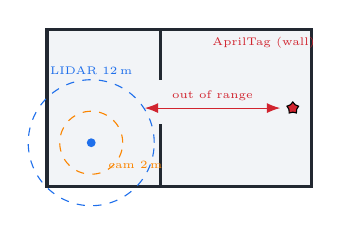
\begin{tikzpicture}[font=\scriptsize,scale=0.80,transform shape]
    \fill[nccblue!6] (0,0) rectangle (4.2,2.5); \draw[very thick,nccdark] (0,0) rectangle (4.2,2.5);
    \draw[very thick,nccdark] (1.8,2.5)--(1.8,1.7);\draw[very thick,nccdark] (1.8,0)--(1.8,1.0);
    \node[star,star points=5,fill=nccred,draw=black,inner sep=1.3pt] at (3.9,1.25){};
    \node[nccred,right] at (2.5,2.28){\tiny AprilTag (wall)};
    \fill[nccsky] (0.7,0.7) circle (2pt);
    \draw[dashed,nccsky] (0.7,0.7) circle (1.0cm);\node[nccsky] at (0.7,1.85){\tiny LIDAR 12\,m};
    \draw[dashed,nccorange](0.7,0.7) circle (0.5cm);\node[nccorange] at (1.4,0.35){\tiny cam 2\,m};
    \draw[{Latex}-{Latex},nccred](1.55,1.25)--(3.7,1.25)node[midway,above]{\tiny out of range};
  \end{tikzpicture}\\
  {\scriptsize The camera-vs-LIDAR gap that the inspection phase closes.}
  \end{column}
  \end{columns}
\end{frame}

% -- Journey --
\begin{frame}{The decision journey - three runs}
  \centering
  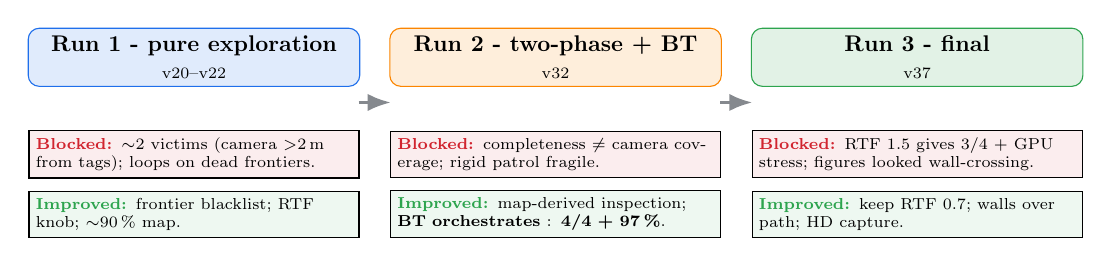
\begin{tikzpicture}[font=\scriptsize,scale=0.82,transform shape]
  \foreach \i/\x/\c/\t/\v in {1/0/nccsky/{Run 1 - pure exploration}/{v20–v22},2/5.6/nccorange/{Run 2 - two-phase + BT}/{v32},3/11.2/nccgreen/{Run 3 - final}/{v37}}{
    \node[draw=\c,fill=\c!14,rounded corners,text width=4.9cm,align=center,font=\bfseries,minimum height=7mm](h\i) at (\x+2.45,4.4){\t\\\normalfont\scriptsize \v};}
  \node[draw,fill=nccred!8,text width=4.9cm,align=left,inner sep=3pt](b1) at (2.45,2.9){\textbf{\color{nccred}Blocked:} $\sim$2 victims (camera $>$2\,m from tags); loops on dead frontiers.};
  \node[draw,fill=nccgreen!8,text width=4.9cm,align=left,inner sep=3pt,below=2mm of b1](i1){\textbf{\color{nccgreen}Improved:} frontier blacklist; RTF knob; $\sim$90\,\% map.};
  \node[draw,fill=nccred!8,text width=4.9cm,align=left,inner sep=3pt](b2) at (8.05,2.9){\textbf{\color{nccred}Blocked:} completeness $\neq$ camera coverage; rigid patrol fragile.};
  \node[draw,fill=nccgreen!8,text width=4.9cm,align=left,inner sep=3pt,below=2mm of b2](i2){\textbf{\color{nccgreen}Improved:} map-derived inspection; \textbf{BT orchestrates} : \textbf{4/4 + 97\,\%}.};
  \node[draw,fill=nccred!8,text width=4.9cm,align=left,inner sep=3pt](b3) at (13.65,2.9){\textbf{\color{nccred}Blocked:} RTF~1.5 gives 3/4 + GPU stress; figures looked wall-crossing.};
  \node[draw,fill=nccgreen!8,text width=4.9cm,align=left,inner sep=3pt,below=2mm of b3](i3){\textbf{\color{nccgreen}Improved:} keep RTF~0.7; walls over path; HD capture.};
  \draw[-{Latex},very thick,nccdark!55] (5.0,3.7)--(5.5,3.7);
  \draw[-{Latex},very thick,nccdark!55] (10.6,3.7)--(11.1,3.7);
  \end{tikzpicture}
  \par\smallskip
  {\footnotesize Two hidden root causes: Nav2 cost discouraged \emph{entering} rooms (coverage); a
  collapsed RTF \emph{starved the camera} (detection). The 2-phase BT then made 4/4 reliable.}
\end{frame}

% -- Results 1 --
\begin{frame}{Results - live algorithms in RViz}
  \centering
  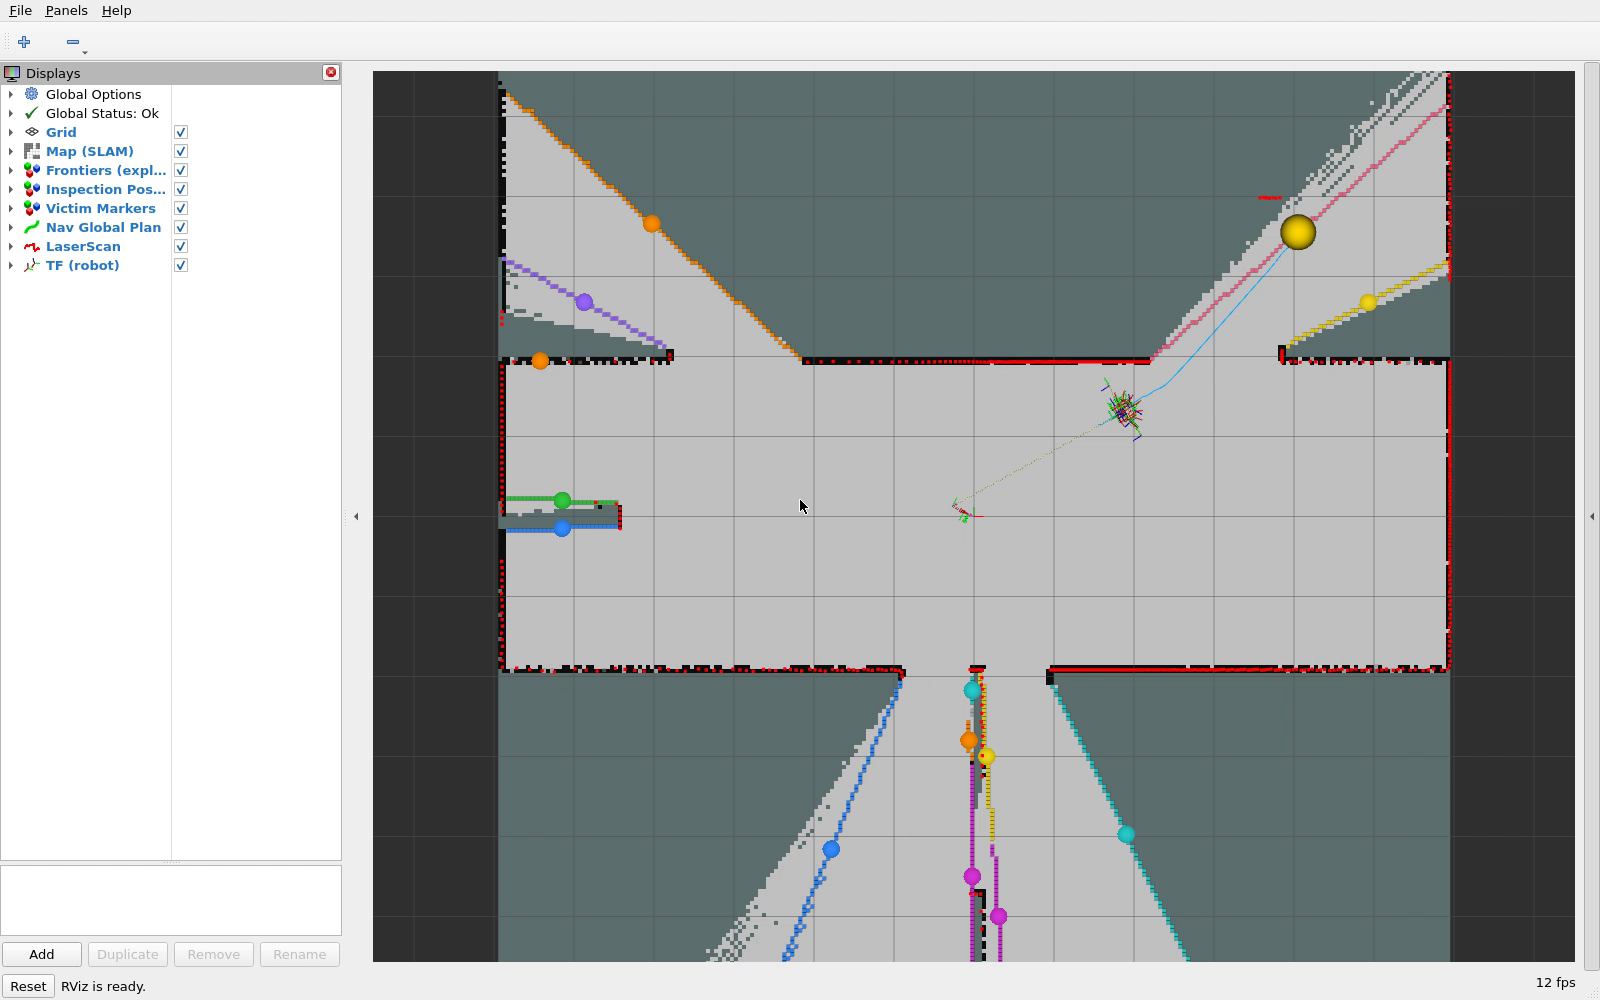
\includegraphics[width=0.275\linewidth]{rviz_seq_1}\hfill
  
\includegraphics[width=0.275\linewidth]{rviz_seq_3}\hfill
  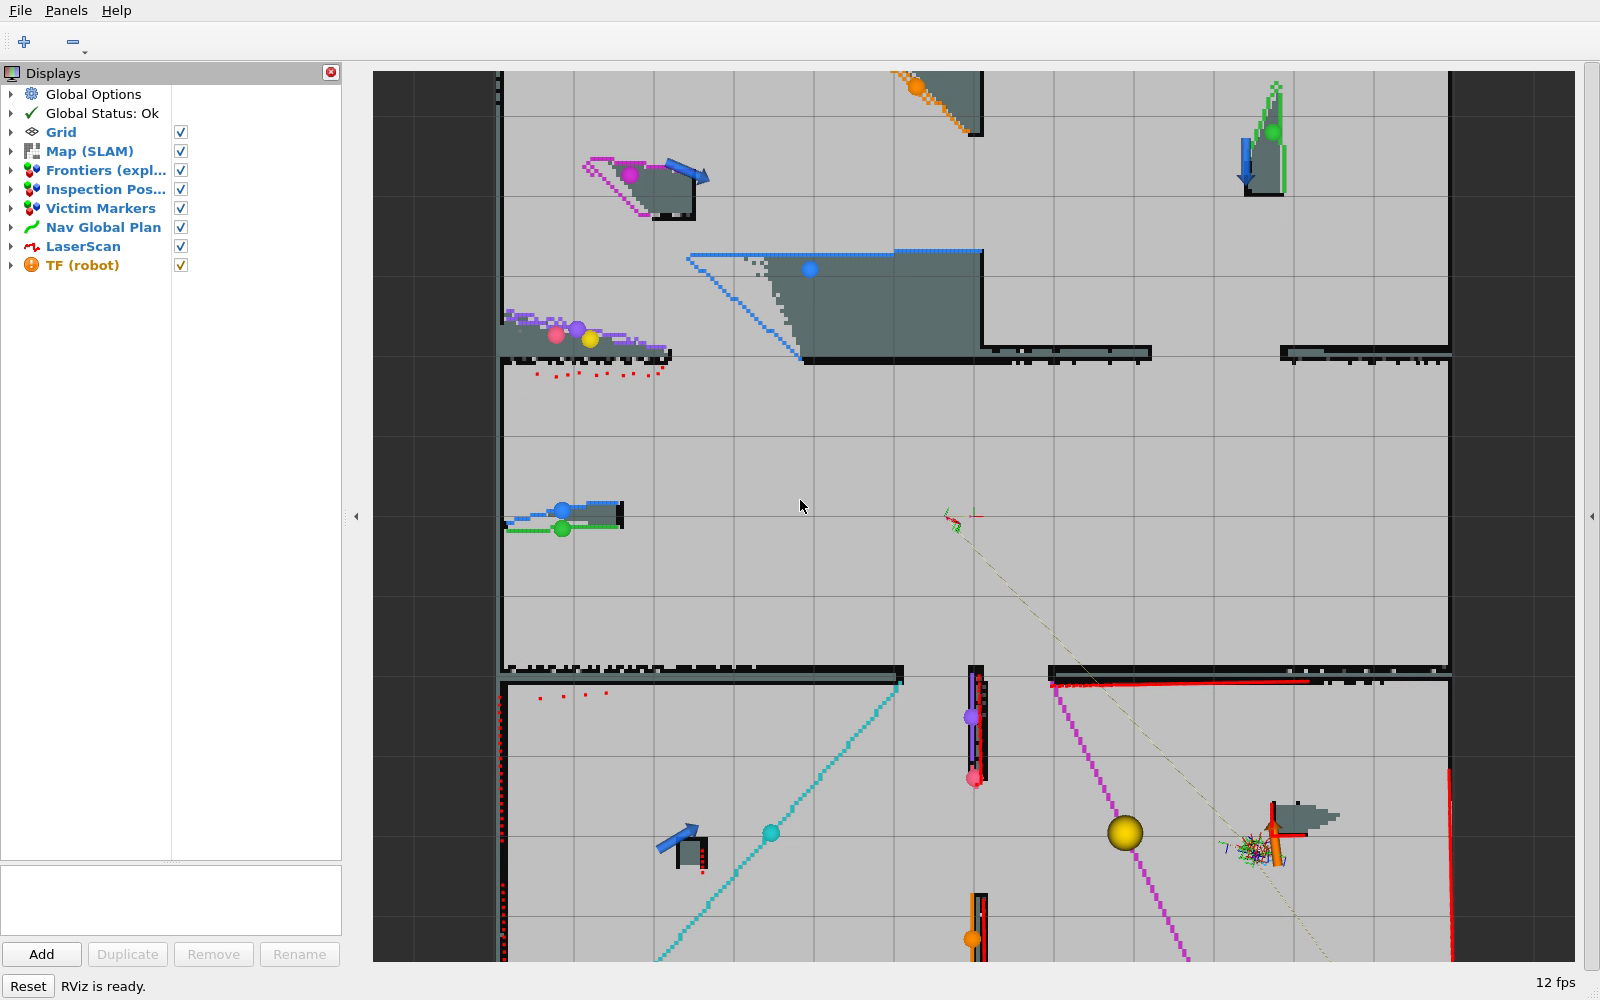
\includegraphics[width=0.275\linewidth]{rviz_seq_4}\\[1pt]
  
\includegraphics[width=0.275\linewidth]{rviz_seq_5}\hfill
  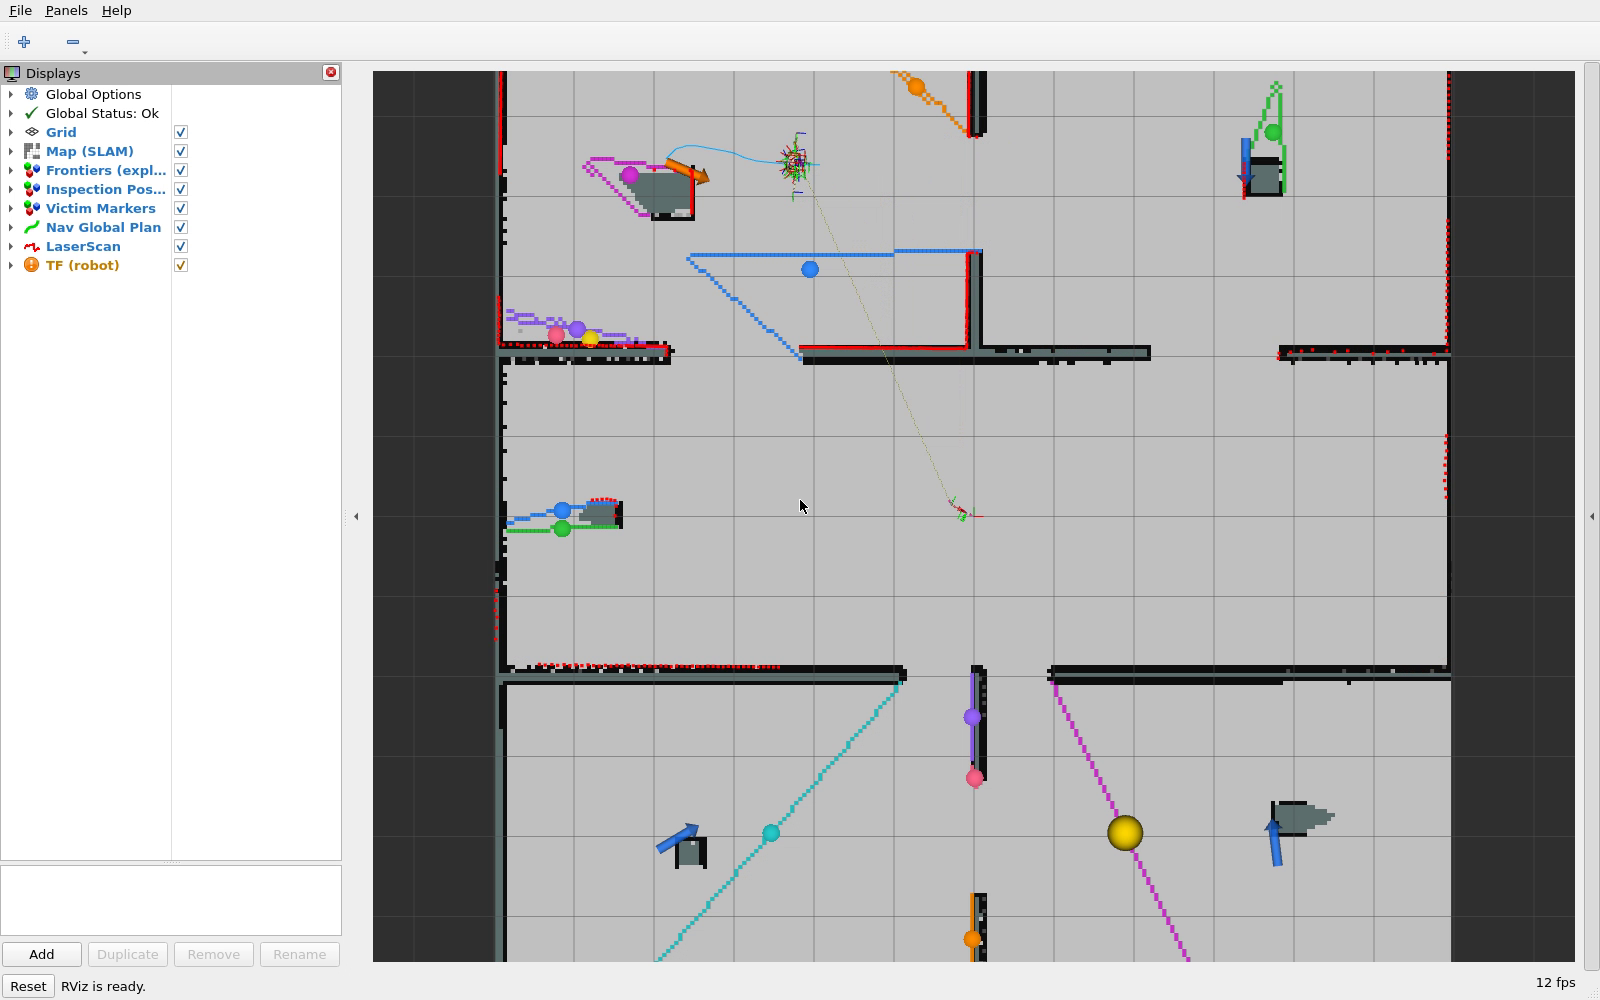
\includegraphics[width=0.275\linewidth]{rviz_seq_6}\hfill
  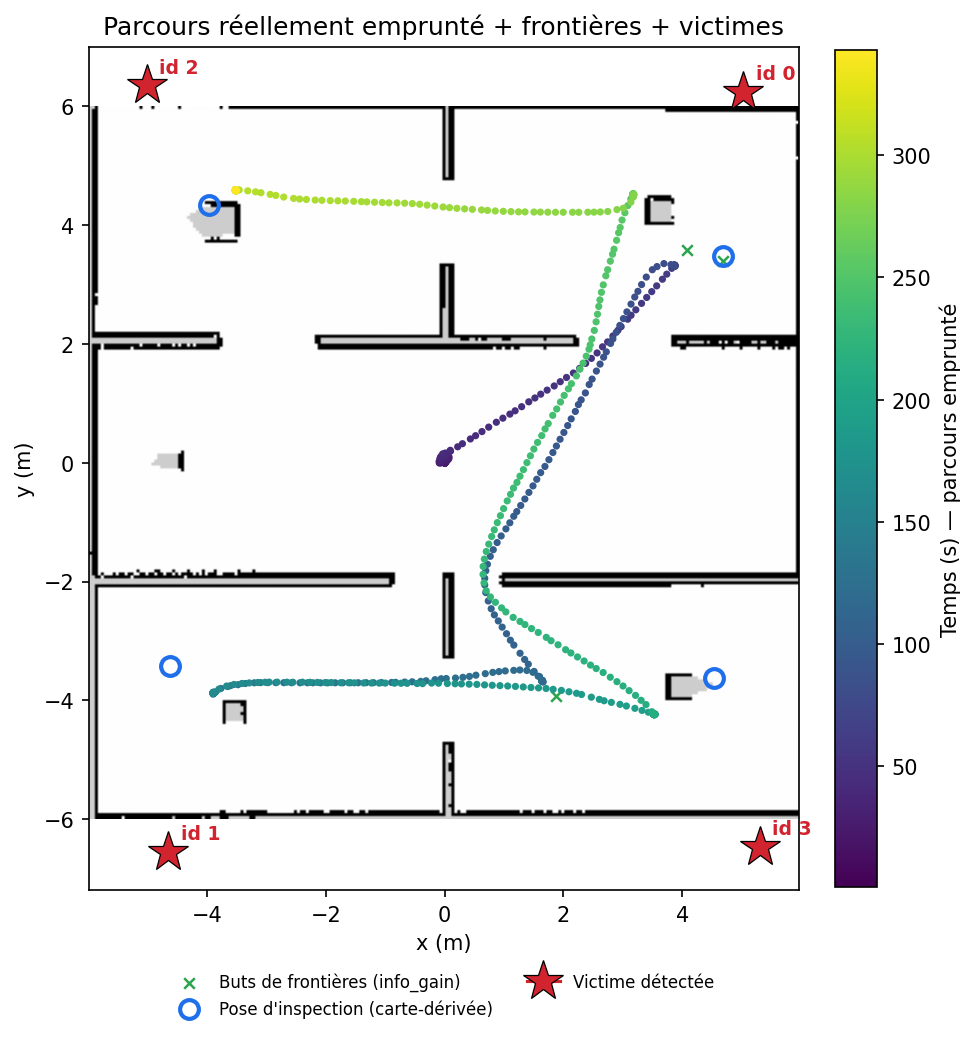
\includegraphics[width=0.275\linewidth]{trajectory_map}
  \par\smallskip
  {\scriptsize Exploration, inspection, four victims; bottom-right: the real map-frame path
  (walls drawn over it, so it visibly threads the doorways - no segment crosses a wall).}
\end{frame}

% -- Seeing the algorithm: Gazebo vs RViz frontiers --
\begin{frame}{Seeing the algorithm: Gazebo (simulator) vs RViz (frontiers)}
  \begin{columns}[c]
  \begin{column}{0.5\linewidth}\centering
  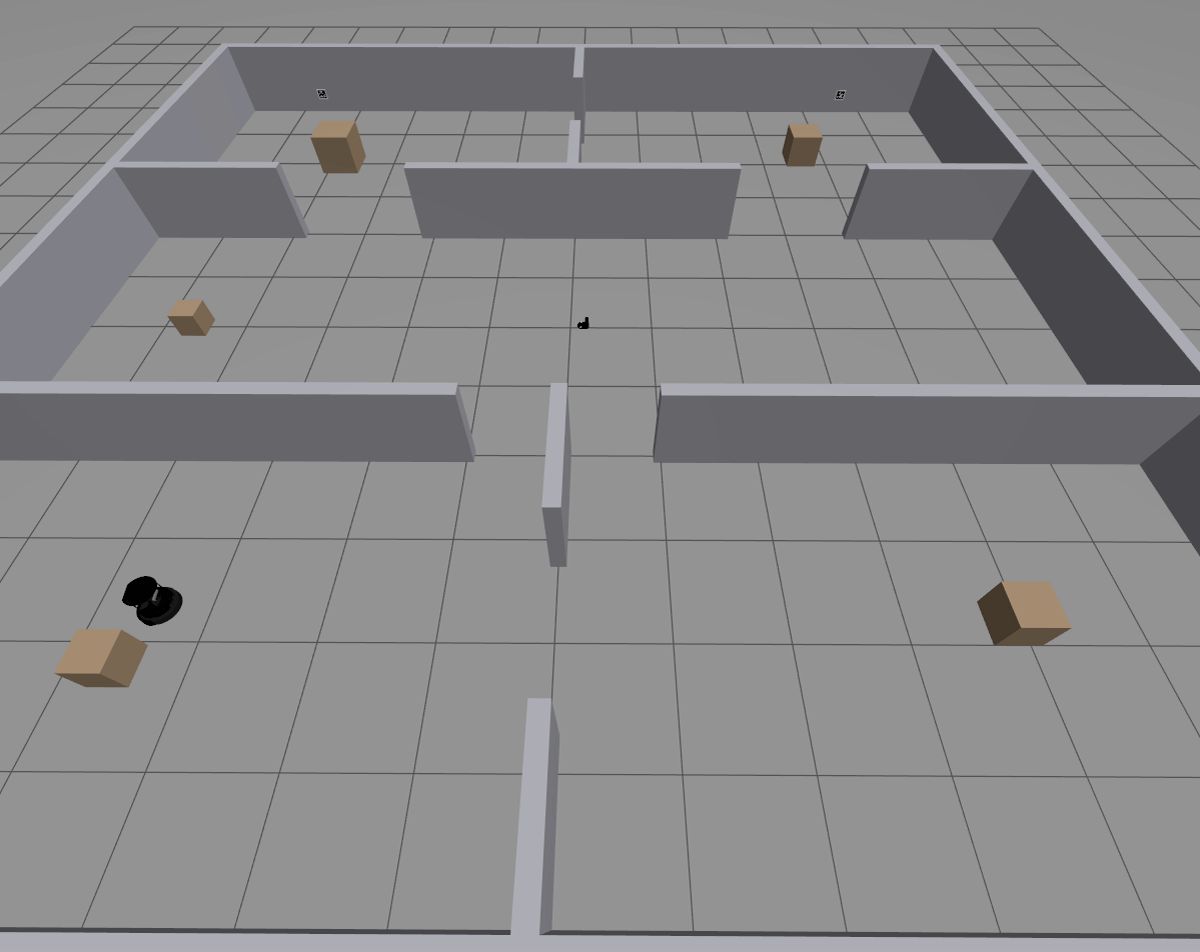
\includegraphics[width=0.90\linewidth]{gazebo_arena}\\[2pt]
  {\scriptsize \textbf{Gazebo} - the simulated arena: walls, victims (AprilTags) and the robot.}
  \end{column}
  \begin{column}{0.5\linewidth}\centering
  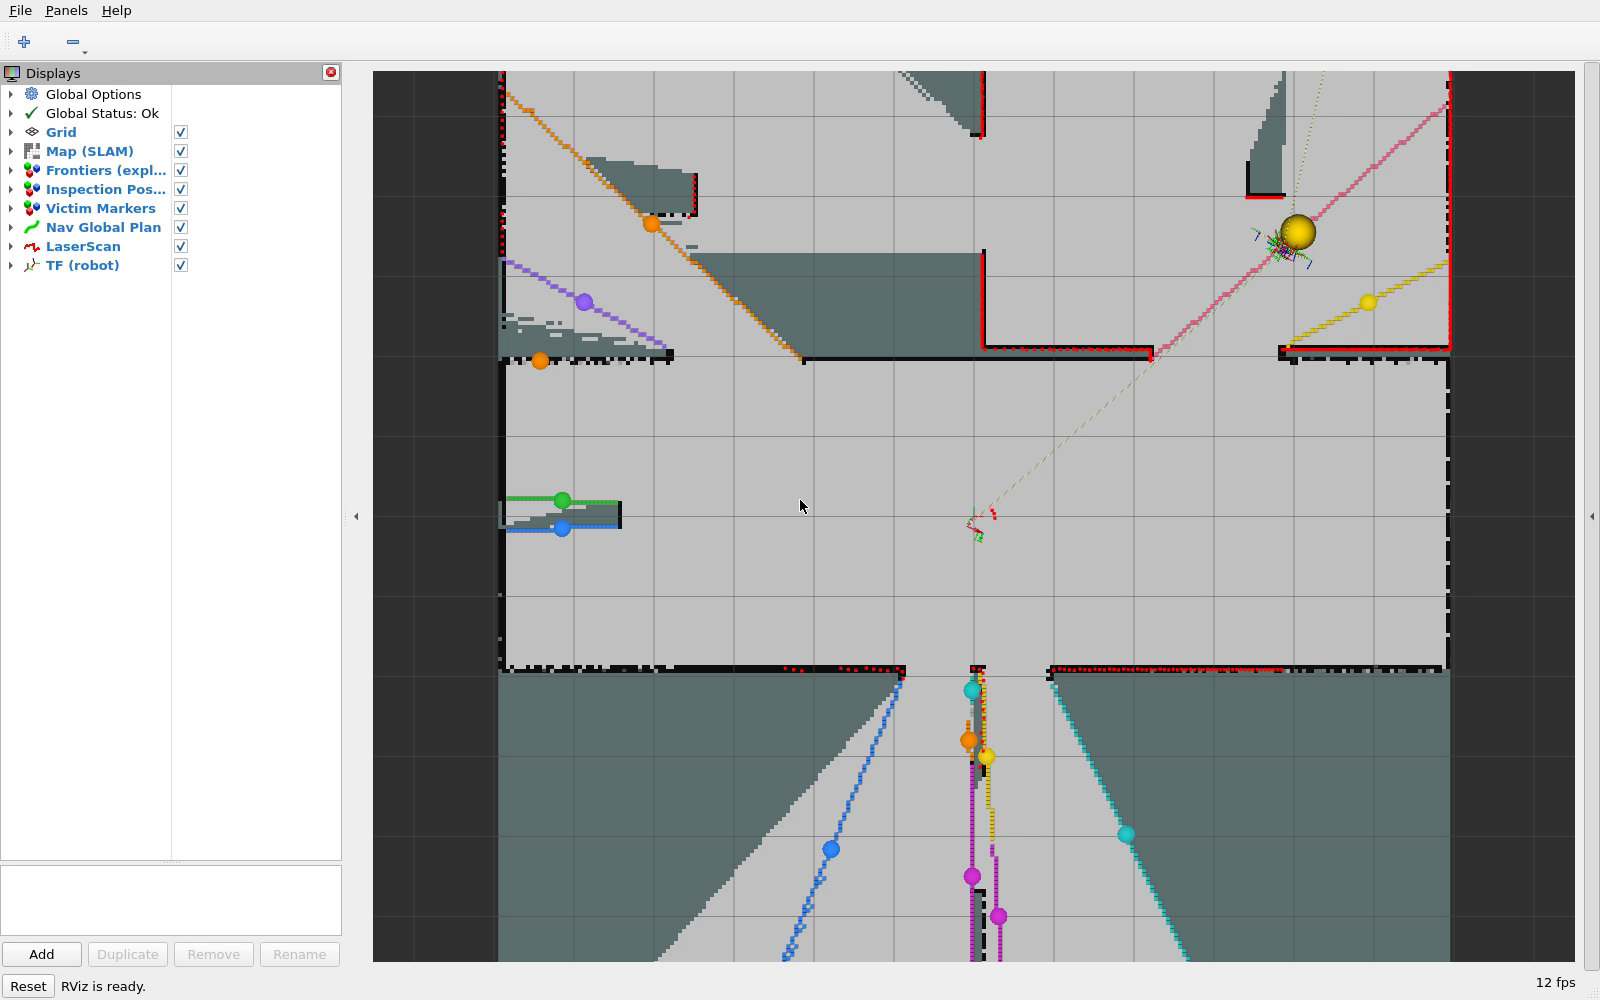
\includegraphics[width=0.90\linewidth]{rviz_frontiers}\\[2pt]
  {\scriptsize \textbf{RViz} - the SLAM map + \emph{frontier cells coloured per cluster}, the goal frontier (yellow) and the Nav2 plan (blue).}
  \end{column}
  \end{columns}
  \smallskip
  {\footnotesize\color{nccblue}\centering As in the labs (CM8): each frontier \emph{cluster} has its own colour, the robot targets the best utility $g=\text{gain}-\lambda\,\text{cost}$, and you \emph{see} the coloured rim eat into the unknown up to $>90\,\%$. Captures: \texttt{gazebo\_capture.mp4} \& \texttt{rviz\_capture.mp4}.}
\end{frame}

% -- Demonstration (video) --
\begin{frame}{Demonstration}
  \centering
  \vfill
  {\large\bfseries \underline{Démo RobotZ}}\\[3mm]
  \href{https://www.youtube.com/watch?v=BKXprWFloFs}{
\includegraphics[width=0.60\linewidth]{youtube_demo.jpg}}\\[3mm]
  {\footnotesize Full-mission video (autonomous run, one click):
  \url{https://www.youtube.com/watch?v=BKXprWFloFs}}
  \vfill
\end{frame}

% -- Bonus: coverage benchmark --
\begin{frame}{Bonus: map coverage - greedy vs information-gain}
  \centering
  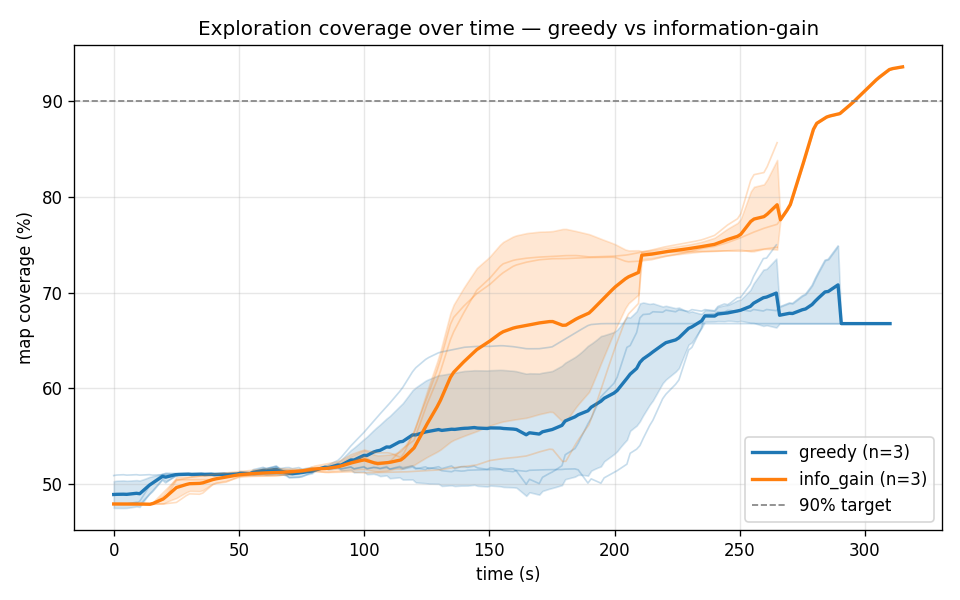
\includegraphics[width=0.62\linewidth]{coverage_over_time}\\[1.5mm]
  {\footnotesize\color{nccblue} Benchmark $n{=}3$: \textbf{information-gain} (orange) reaches the 90\,\%
  target; \textbf{greedy} (blue) plateaus at $\sim$67--70\,\% and never reaches it - it commits to opening
  whole rooms (more unknown per metre), whereas greedy nibbles locally and stalls.}
\end{frame}

% -- Results 2 --
\begin{frame}{Results - coverage, map and conformity}
  \begin{columns}[c]
  \begin{column}{0.5\linewidth}\centering
  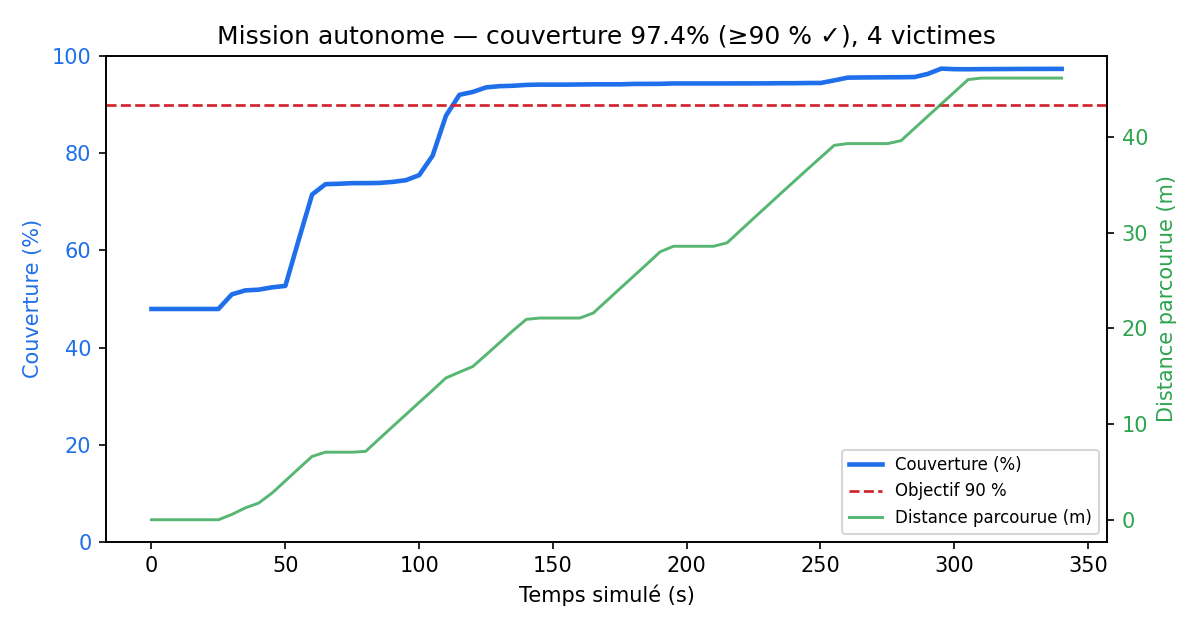
\includegraphics[width=0.96\linewidth]{coverage_curve}\\{\scriptsize Coverage \& path vs.\ time, 90\,\% target.}
  \end{column}
  \begin{column}{0.5\linewidth}\centering
  
\includegraphics[width=0.72\linewidth]{mission_map}\\{\scriptsize Final map: 4 victims + autonomous inspection tour.}
  \end{column}
  \end{columns}
  \smallskip
  {\footnotesize\color{nccblue}\centering \textbf{97.35\,\% coverage $\cdot$ 4/4 victims $\cdot$ annotated map $\cdot$ logged trajectory} - one click, fully autonomous.}
\end{frame}

% -- Team / git --
\begin{frame}{Team and collaboration}
  \begin{columns}[T]
  \begin{column}{0.52\linewidth}
  \footnotesize
  Per-member \texttt{dev/*} branches merged into \texttt{dev/bl} (integration):
  \begin{itemize}
    \item \textbf{Yimou} - exploration, SLAM/Nav2, perception core
    \item \textbf{Julien} - BT decision, infra (WSL/GPU/RTF), results, integration
    \item \textbf{Hugo} - world / arena / AprilTag targets
    \item \textbf{Paul} - perception/detection support, testing
  \end{itemize}
  \end{column}
  \begin{column}{0.46\linewidth}\centering
  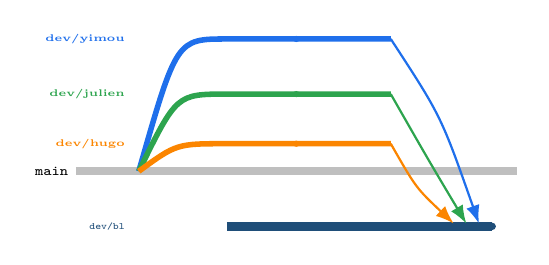
\begin{tikzpicture}[font=\scriptsize,xscale=0.8,yscale=0.7,transform shape]
    \draw[gray!50,line width=3pt] (0,0)--(7,0);\node[left] at (0,0){\texttt{main}};
    \foreach \y/\n/\c in {2.4/{dev/yimou}/nccsky,1.4/{dev/julien}/nccgreen,0.5/{dev/hugo}/nccorange}{
      \draw[\c,line width=2pt] (1,0) .. controls (1.6,\y) .. (2.4,\y) -- (5,\y);
      \node[\c,left,font=\tiny\bfseries] at (0.9,\y){\n};
      \fill[\c] (3.5,\y) circle (1.6pt);}
    \draw[nccblue,line width=3pt] (2.4,-1.0)--(6.6,-1.0);\node[nccblue,left,font=\tiny\bfseries] at (0.9,-1.0){\texttt{dev/bl}};
    \draw[-{Latex},nccsky,thick] (5,2.4) .. controls (5.8,1) .. (6.4,-0.95);
    \draw[-{Latex},nccgreen,thick] (5,1.4) .. controls (5.6,0.2) .. (6.2,-0.95);
    \draw[-{Latex},nccorange,thick] (5,0.5) .. controls (5.4,-0.3) .. (6.0,-0.95);
    \fill[nccblue] (6.6,-1.0) circle (2pt);
  \end{tikzpicture}\\
  {\scriptsize Three workstreams to \texttt{bl} integration.}
  \end{column}
  \end{columns}
\end{frame}

% -- Lessons --
\begin{frame}{Lessons learned}
  \begin{itemize}
    \item \textbf{Measure before prescribing} - ``obvious'' causes (memory, Windows Update) were wrong twice; event logs found the real ones (GPU TDR, a starved camera).
    \item \textbf{One fix reveals the next} - victim detection crossed six stacked causes.
    \item \textbf{Robust beats rigid} - adaptive exploration + 360$^\circ$ sweep beat a fixed patrol; the inspector also recovers a pose another machine cannot reach (wait for the costmap, fall back into the room) - \emph{cross-machine robustness}.
    \item \textbf{Conformity by design} - a BT that \emph{orchestrates} (not just supervises) meets the assignment in spirit, not only in letter.
  \end{itemize}
  \vfill
  {\footnotesize\color{nccblue}Timeline: L13 kick-off $\cdot$ L14 architecture $\cdot$ L15 nodes/SLAM $\cdot$ L16 BT+perception $\cdot$ L17 integration/benchmark $\cdot$ L18 two-phase, final run, report.}
\end{frame}

% -- Thanks --
\begin{frame}[plain]
  \centering
  \vfill
  {\Large\color{nccblue}\textbf{Thank you - Questions?}}\\[10pt]
  {\small We warmly thank \textbf{Zhi Yan}, Teacher-Researcher at ENSTA,\\ for the IA712 course and guidance.}\\[14pt]
  {\footnotesize \texttt{https://github.com/YiZeems/autonomous-search-and-rescue}}\\[4pt]
  {\scriptsize Julien GIMENEZ $\cdot$ Hugo FANCHINI $\cdot$ Paul CINTRA $\cdot$ Yimou ZHANG}
  \vfill
\end{frame}

\end{document}
